\section{Composites}
\label{sec:composites}

Los composites definen cómo se combinan visualmente las dos fuentes de vídeo activas
(bus A y bus B) en el fotograma de salida. Voctomix implementa los composites mediante
el elemento GStreamer \texttt{compositor}, que sitúa y escala cada fuente de acuerdo
con los parámetros geométricos definidos en la sección \texttt{[composites]} del
fichero de configuración INI. La modificación de estos parámetros en tiempo real
permite transiciones suaves entre composites sin generar fotogramas corruptos.

Los composites disponibles en Voctomix 2.0 son los siguientes:

La figura~\ref{fig:composites_diagrama} ilustra la disposición visual de las dos
fuentes (A en naranja, B en azul) en cada uno de los composites principales.

\begin{figure}[H]
  \centering
  % W=3.2, H=1.8, gap=0.7 → offsets: 0, 3.9, 7.8, 11.7
  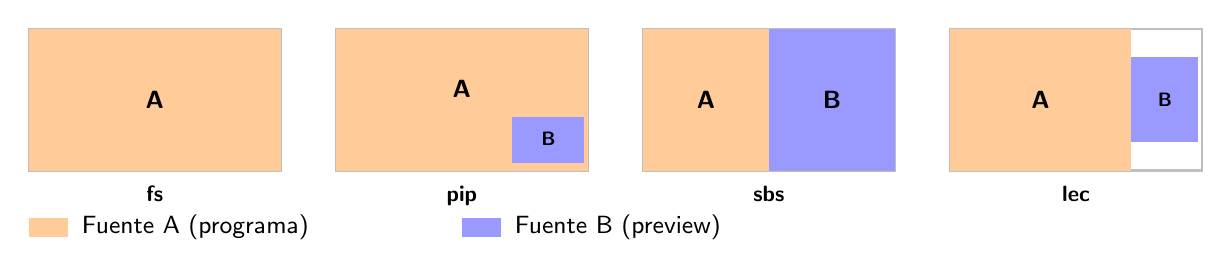
\begin{tikzpicture}[font=\sffamily\small]

    % ─────────── Full Screen (ox=0) ────────────────────────────────────
    \draw[thick, gray!50] (0,0) rectangle (3.2,1.8);
    \fill[orange!40] (0,0) rectangle (3.2,1.8);
    \node[font=\sffamily\bfseries\small] at (1.6,0.9) {A};
    \node[font=\sffamily\footnotesize, below=2pt] at (1.6,0) {\textbf{fs}};

    % ─────────── Picture in Picture (ox=3.9) ───────────────────────────
    \draw[thick, gray!50] (3.9,0) rectangle (7.1,1.8);
    \fill[orange!40] (3.9,0) rectangle (7.1,1.8);
    \node[font=\sffamily\bfseries\small] at (5.5,1.04) {A};
    \fill[blue!40] (6.14,0.10) rectangle (7.05,0.684);
    \node[font=\sffamily\bfseries\scriptsize] at (6.60,0.40) {B};
    \node[font=\sffamily\footnotesize, below=2pt] at (5.5,0) {\textbf{pip}};

    % ─────────── Side by Side (ox=7.8) ─────────────────────────────────
    \draw[thick, gray!50] (7.8,0) rectangle (11.0,1.8);
    \fill[orange!40] (7.8,0) rectangle (9.4,1.8);
    \fill[blue!40]   (9.4,0) rectangle (11.0,1.8);
    \node[font=\sffamily\bfseries\small] at (8.6,0.9) {A};
    \node[font=\sffamily\bfseries\small] at (10.2,0.9) {B};
    \node[font=\sffamily\footnotesize, below=2pt] at (9.4,0) {\textbf{sbs}};

    % ─────────── Lecture (ox=11.7) ─────────────────────────────────────
    \draw[thick, gray!50] (11.7,0) rectangle (14.9,1.8);
    \fill[orange!40] (11.7,0) rectangle (14.004,1.8);
    \fill[blue!40]   (14.004,0.36) rectangle (14.85,1.44);
    \node[font=\sffamily\bfseries\small] at (12.85,0.9) {A};
    \node[font=\sffamily\bfseries\scriptsize] at (14.43,0.9) {B};
    \node[font=\sffamily\footnotesize, below=2pt] at (13.3,0) {\textbf{lec}};

    % ─────────── leyenda ───────────────────────────────────────────────
    \fill[orange!40] (0,-0.85) rectangle (0.5,-0.60);
    \node[right, font=\sffamily\small] at (0.55,-0.72) {Fuente A (programa)};
    \fill[blue!40] (5.5,-0.85) rectangle (6.0,-0.60);
    \node[right, font=\sffamily\small] at (6.05,-0.72) {Fuente B (preview)};
  \end{tikzpicture}
  \caption{Disposición visual de las fuentes A y B en los cuatro composites
           principales de Voctomix~2.0: pantalla completa (\texttt{fs}),
           imagen en imagen (\texttt{pip}), lado a lado (\texttt{sbs}) y
           conferencia (\texttt{lec}).}
  \label{fig:composites_diagrama}
\end{figure}

\subsection{Full Screen (fs)}

La fuente A ocupa toda la pantalla y la fuente B queda oculta (alpha = 0). Es el modo
por defecto de una realización convencional: el realizador selecciona una fuente y la
emite a pantalla completa. Resulta adecuado para la emisión de una ponencia individual,
una demostración en pantalla o cualquier situación en la que una única fuente deba
ocupar todo el encuadre.

\subsection{Picture in Picture (pip)}

La fuente A se muestra a pantalla completa mientras la fuente B aparece reducida en
una esquina del encuadre (tipicamente la esquina inferior derecha), a una escala
aproximada del 27\% del ancho del fotograma. Es el composite clásico de ``ponente con
presentación'': la cámara del ponente ocupa la pantalla completa y las diapositivas
aparecen en la esquina, o viceversa. Puede configurarse con \texttt{mirror=true} para
que la fuente A se invierta horizontalmente, útil cuando la cámara tiene la imagen
especular por la disposición del equipo.

\subsection{Side by Side (sbs)}

Ambas fuentes se muestran a igual tamaño, situadas una junto a la otra y ocupando
cada una aproximadamente la mitad del fotograma. Es útil para comparaciones visuales,
debates con dos participantes o para mostrar simultáneamente la cámara del ponente y
sus diapositivas con el mismo peso visual.

\subsection{Lecture (lec)}

La fuente A ocupa la mayor parte del encuadre (aproximadamente el 75\%) mientras que
la fuente B aparece reducida en la parte derecha. Este composite está específicamente
diseñado para retransmisiones de ponencias o clases: las diapositivas (fuente A)
dominan el encuadre y la cámara del ponente (fuente B) aparece en un recuadro lateral
de menor tamaño, manteniendo siempre la legibilidad del contenido proyectado.

La variante \texttt{lec\_43} está concebida para acomodar contenido con relación de
aspecto 4:3 (como proyectores antiguos o capturas de escritorio con resolución
1024\texttimes{}768) en un encuadre 16:9. En la versión original del repositorio, esta
variante aplicaba un recorte del 31\% mediante el parámetro \texttt{crop-a=0.125/0}
que destruía el encuadre completo cuando la fuente era nativa 16:9. Se corrigió
redefiniendo los parámetros de posición y escala en la sección \texttt{[composites]}
del fichero INI para eliminar el recorte y ajustar la ventana secundaria de forma que
encaje perfectamente a la derecha sin desbordarse del fotograma.

\subsection{Mirror}

Aunque no es un composite independiente sino una propiedad disponible en varios de
los anteriores (\texttt{mirror=true} en \texttt{pip}, \texttt{lec} y \texttt{fs-pip}),
el efecto espejo permite invertir horizontalmente la fuente A o B en el composite. Esto
es necesario cuando la señal de cámara llega especularmente invertida, como puede
ocurrir con ciertos modelos de cámaras web o cuando la cámara está orientada de forma
atípica. Al activar el mirror desde el fichero de configuración, el núcleo aplica la
inversión directamente en el compositor de GStreamer sin coste adicional.

\begin{figure}[H]
  \centering
  \fbox{\begin{minipage}{0.85\textwidth}\centering\vspace{1.2cm}
    \textit{[IMAGEN PENDIENTE: captura del selector de composites en voctogui,}\\
    \textit{mostrando los botones FULL SCREEN, PIP, SIDE BY SIDE y LECTURE]}\\
    \textit{con el composite activo resaltado.}\\[4pt]
    \textit{Guardar como \texttt{figuras/panel\_composites.png} y enviar.}
    \vspace{1.2cm}
  \end{minipage}}
  \caption{Selector de modos de composite en la interfaz de Voctomix~2.0.}
  \label{fig:panel_composites}
\end{figure}
